\tikzset{%
  every neuron/.style={
    circle,
    draw,
    minimum size=1cm
  },
  neuron missing/.style={
    draw=none,
    scale=4,
    text height=0.333cm,
    execute at begin node=\color{black}$\vdots$
  },
}

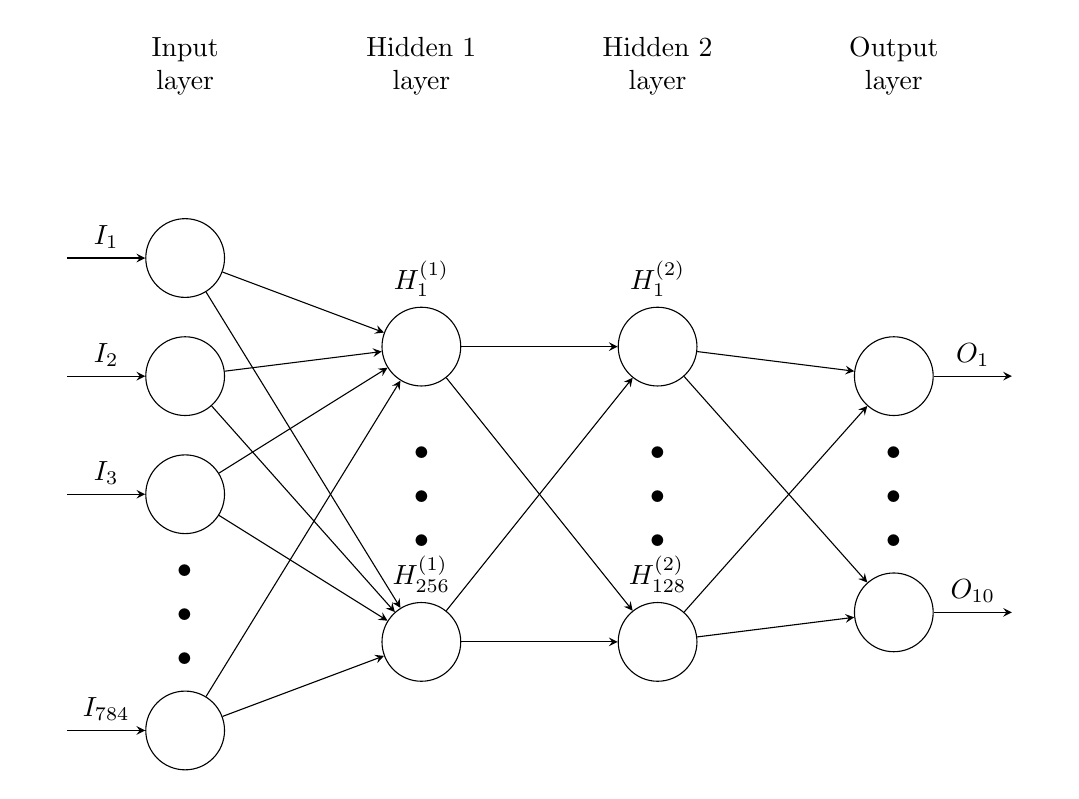
\begin{tikzpicture}[x=1.5cm, y=1.5cm, >=stealth]

% INPUT layer
\foreach \m/\l [count=\y] in {1,2,3,missing,4}
  \node [every neuron/.try, neuron \m/.try] 
    (input-\m) at (0,2.5-\y) {};

% FIRST HIDDEN layer
\foreach \m [count=\y] in {1,missing,2}
  \node [every neuron/.try, neuron \m/.try ] 
    (hiddenA-\m) at (2,2-\y*1.25) {};

% SECOND HIDDEN layer
\foreach \m [count=\y] in {1,missing,2}
  \node [every neuron/.try, neuron \m/.try ] 
    (hiddenB-\m) at (4,2-\y*1.25) {};

% OUTPUT layer
\foreach \m [count=\y] in {1,missing,2}
  \node [every neuron/.try, neuron \m/.try ] 
    (output-\m) at (6,1.5-\y) {};

% INPUT labels
\foreach \l [count=\i] in {1,2,3,{784}}
  \draw [<-] (input-\i) -- ++(-1,0)
    node [above, midway] {$I_{\l}$};

% Hidden labels
\foreach \l [count=\i] in {1,{256}}
  \node [above] at (hiddenA-\i.north) {$H^{(1)}_{\l}$};

\foreach \l [count=\i] in {1,{128}}
  \node [above] at (hiddenB-\i.north) {$H^{(2)}_{\l}$};

% Output labels
\foreach \l [count=\i] in {1,{10}}
  \draw [->] (output-\i) -- ++(1,0)
    node [above, midway] {$O_{\l}$};

% Connections: input -> hiddenA
\foreach \i in {1,...,4}
  \foreach \j in {1,...,2}
    \draw [->] (input-\i) -- (hiddenA-\j);

% Connections: hiddenA -> hiddenB
\foreach \i in {1,...,2}
  \foreach \j in {1,...,2}
    \draw [->] (hiddenA-\i) -- (hiddenB-\j);

% Connections: hiddenB -> output
\foreach \i in {1,...,2}
  \foreach \j in {1,...,2}
    \draw [->] (hiddenB-\i) -- (output-\j);

% LAYER labels
\foreach \l [count=\x from 0] in {Input, Hidden 1, Hidden 2, Output}
  \node [align=center, above] at (\x*2,2.8) {\l \\ layer};

\end{tikzpicture}
